\documentclass[12pt]{article}
\usepackage[margin=1in]{geometry} 
\usepackage{amsmath,amsthm,amssymb,amsfonts}
\usepackage{placeins}
\usepackage{mathtools, eucal}
 

 
\begin{document}
 
%\renewcommand{\qedsymbol}{\filledbox}
%Good resources for looking up how to do stuff:
%Binary operators: http://www.access2science.com/latex/Binary.html
%General help: http://en.wikibooks.org/wiki/LaTeX/Mathematics
%Or just google stuff
 
\title{Homework 2 Solutions}
\author{Zheming Gao}
\maketitle

\section*{Problem 1.1}

Solutions: 
\begin{enumerate}
\item 

Let $x_2 = x_2^+ - x_2^-$ and $x_2 ^+, x_2^- \geqslant 0$.
And add slack variables $\xi_1, \xi_2$ on the first and the second constraint respectively.

\begin{equation*}
\begin{aligned}
\text{Minimize} \quad & 4x_1 + \sqrt{2}x_2^+ - \sqrt{2}x_2^- - 0.35 x_3 \\
\text{subject\  to} \quad & -0.001x_1 + 200 x_2^+ - 200 x_2^- - \xi_1 = 7\sqrt{261} \\
& 7.07 x_2^+ - 7.07 x_2^- - 2.62 x_3 + \xi_2 = -4 \\
& x_1, x_2^+, x_2^-, x_3, \xi_1, \xi_2 \geqslant 0
\end{aligned}
\end{equation*}

\item

Let $a_1 = x_1 - 20$, $a_3 = x_3 + 15$, then $a_1, a_3 \geqslant 0$, and $x_1 = a_1 + 20, x_3 = a_3 - 15$.

Add a slack variable $\xi_1$ on the second constraint. The standard form is

\begin{equation*}
\begin{aligned}
\text{Minimize} \quad & 3.1a_1 - 2\sqrt{2}x_2 + a_3 \\
\text{subject\  to} \quad & 100a_1 - 20 x_2 = -1993 \\
& -11a_1 - 7\pi x_2 - 2a_3 + \xi_1 = 590\\
& a_1, x_2, a_3, \xi_1 \geqslant 0
\end{aligned}
\end{equation*}

Notice that the objective function should have been $3.1a_1 - 2\sqrt{2}x_2 + a_3 + 47$, which is an affine function. But to make it a linear function, we eliminate $+47$. We will obtain the same optimal solutions but will need to add $47$ on the optimal value.


\item

Since $x_3 \leqslant 10$, $10 - x_3 \geqslant 0$. Let $a_3 = 10 - x_3$, then $a_3 \geqslant 0$ and $x_3 = 10 - a_3$.
Let $x_1 = x_1^+ - x_1^-$, where $x_1^+, x_1^- \geqslant 0$. Add slack variables on each constraint and the standard form is the following,

\begin{equation*}
\begin{aligned}
\text{Minimize} \quad & -x_1^+ + x_1^- - 3x_2 - 2a_3 (+ 20) \\
\text{subject\  to} \quad & 3x_1^+ - 3x_1^- - 5x_2 - \xi_1 = -2 \\
& 3x_1^+ - 3x_1^- - 5x_2 + \xi_2 = 15\\
& -5x_1^+ + 5x_1^- + 20x_2 - \xi_3 = 11 \\
& -5x_1^+ + 5x_1^- + 20x_2 + \xi_4 = 40 \\
& x_1^+, x_1^-, x_2, a_3, \xi_i (i = 1,\dots, 4)  \geqslant 0
\end{aligned}
\end{equation*}

\end{enumerate}

\section*{Problem 1.2}
\begin{enumerate}
\item[a)]

Let $x_1 = x_1^+ - x_1^-$, where $x_1^+, x_1^- \geqslant 0$. The standard form is the following,

\begin{equation*}
\begin{aligned}
\text{Minimize} \quad & 2x_1^+ - 2x_1^- + 6x_2 + 8x_3 \\
\text{subject\  to} \quad & x_1^+ - x_1^- + 2x_2 + x_3 = 5 \\
& 4x_1^+ - 4x_1^-  + 2x_3 = 12\\
& x_1^+, x_1^-, x_2, x_3 \geqslant 0
\end{aligned}
\end{equation*}

\item[b)]
From the first constraint, solve $x_1$ as $x_1 = 5 - 2x_2 - x_3$. Plug it into the objective function and also the second constraint, then reform the LP problem as the following,

\begin{equation*}
\begin{aligned}
\text{Minimize} \quad & 2x_2 + 6x_3 (+10)\\
\text{subject\  to} \quad & -2x_2 - 2x_3 = -8 \\
& x_2, x_3 \geqslant 0
\end{aligned}
\end{equation*}

\item[c)]
It is already in the standard form.

\item[d)]

Use graphic method to solve the problem. Optimal value is $z* = 18$ and the optimal solution is $x* = (x_2^*, x_3^*) = (4, 0)$.

\FloatBarrier

\begin{figure}[htpb]
  \caption{Problem 1.2 (d)}
  \centering
    \includegraphics[width=0.5\textwidth]{fig1.pdf}
\end{figure}

\FloatBarrier



\end{enumerate}


\section*{Problem 1.3}

\begin{enumerate}
\item[a)]

No. Because there is a nonlinear term $x_1^2$ in the objective function and the first constraint.

\item[b)]

Yes. Use the first constraint, solve $x_1^2$ and get $x_1^2 = x_2$. Plug it into the objective function and get 

\begin{equation*}
\begin{aligned}
\text{Minimize} \quad & 2x_2 + 4x_3 \\
\text{subject\  to} \quad & 2x_2 + 4x_3 \geqslant 4 \\
& x_1, x_3 \geqslant 0, x_2 \geqslant 2
\end{aligned}
\end{equation*}


\item[c)]

Use the similar technique in problem 1.1 and 1.2. Let $a_2 = x_2 - 2$. Then $a_2 \geqslant 0$, and $x_2 = a_2 + 2$. Add a slack variable on the constraint. 

\begin{equation*}
\begin{aligned}
\text{Minimize} \quad & 2a_2 + 4x_3 (+ 4) \\
\text{subject\  to} \quad & 2a_2 + 4x_3 - \xi = 0 \\
& x_1, a_2, x_3, \xi \geqslant 0
\end{aligned}
\end{equation*}

\item[d)]

Yes. To solve the LP problem, use graphic method. The optimal solution is $x^* = (x_1^*, x_2^*, x_3^*, x_4^*)^T = (\sqrt{2}, 2, 0, 0)^T$. Optimal value is $z^* = 4$.

\FloatBarrier

\begin{figure}[htpb]
  \caption{Problem 1.3 (d)}
  \centering
    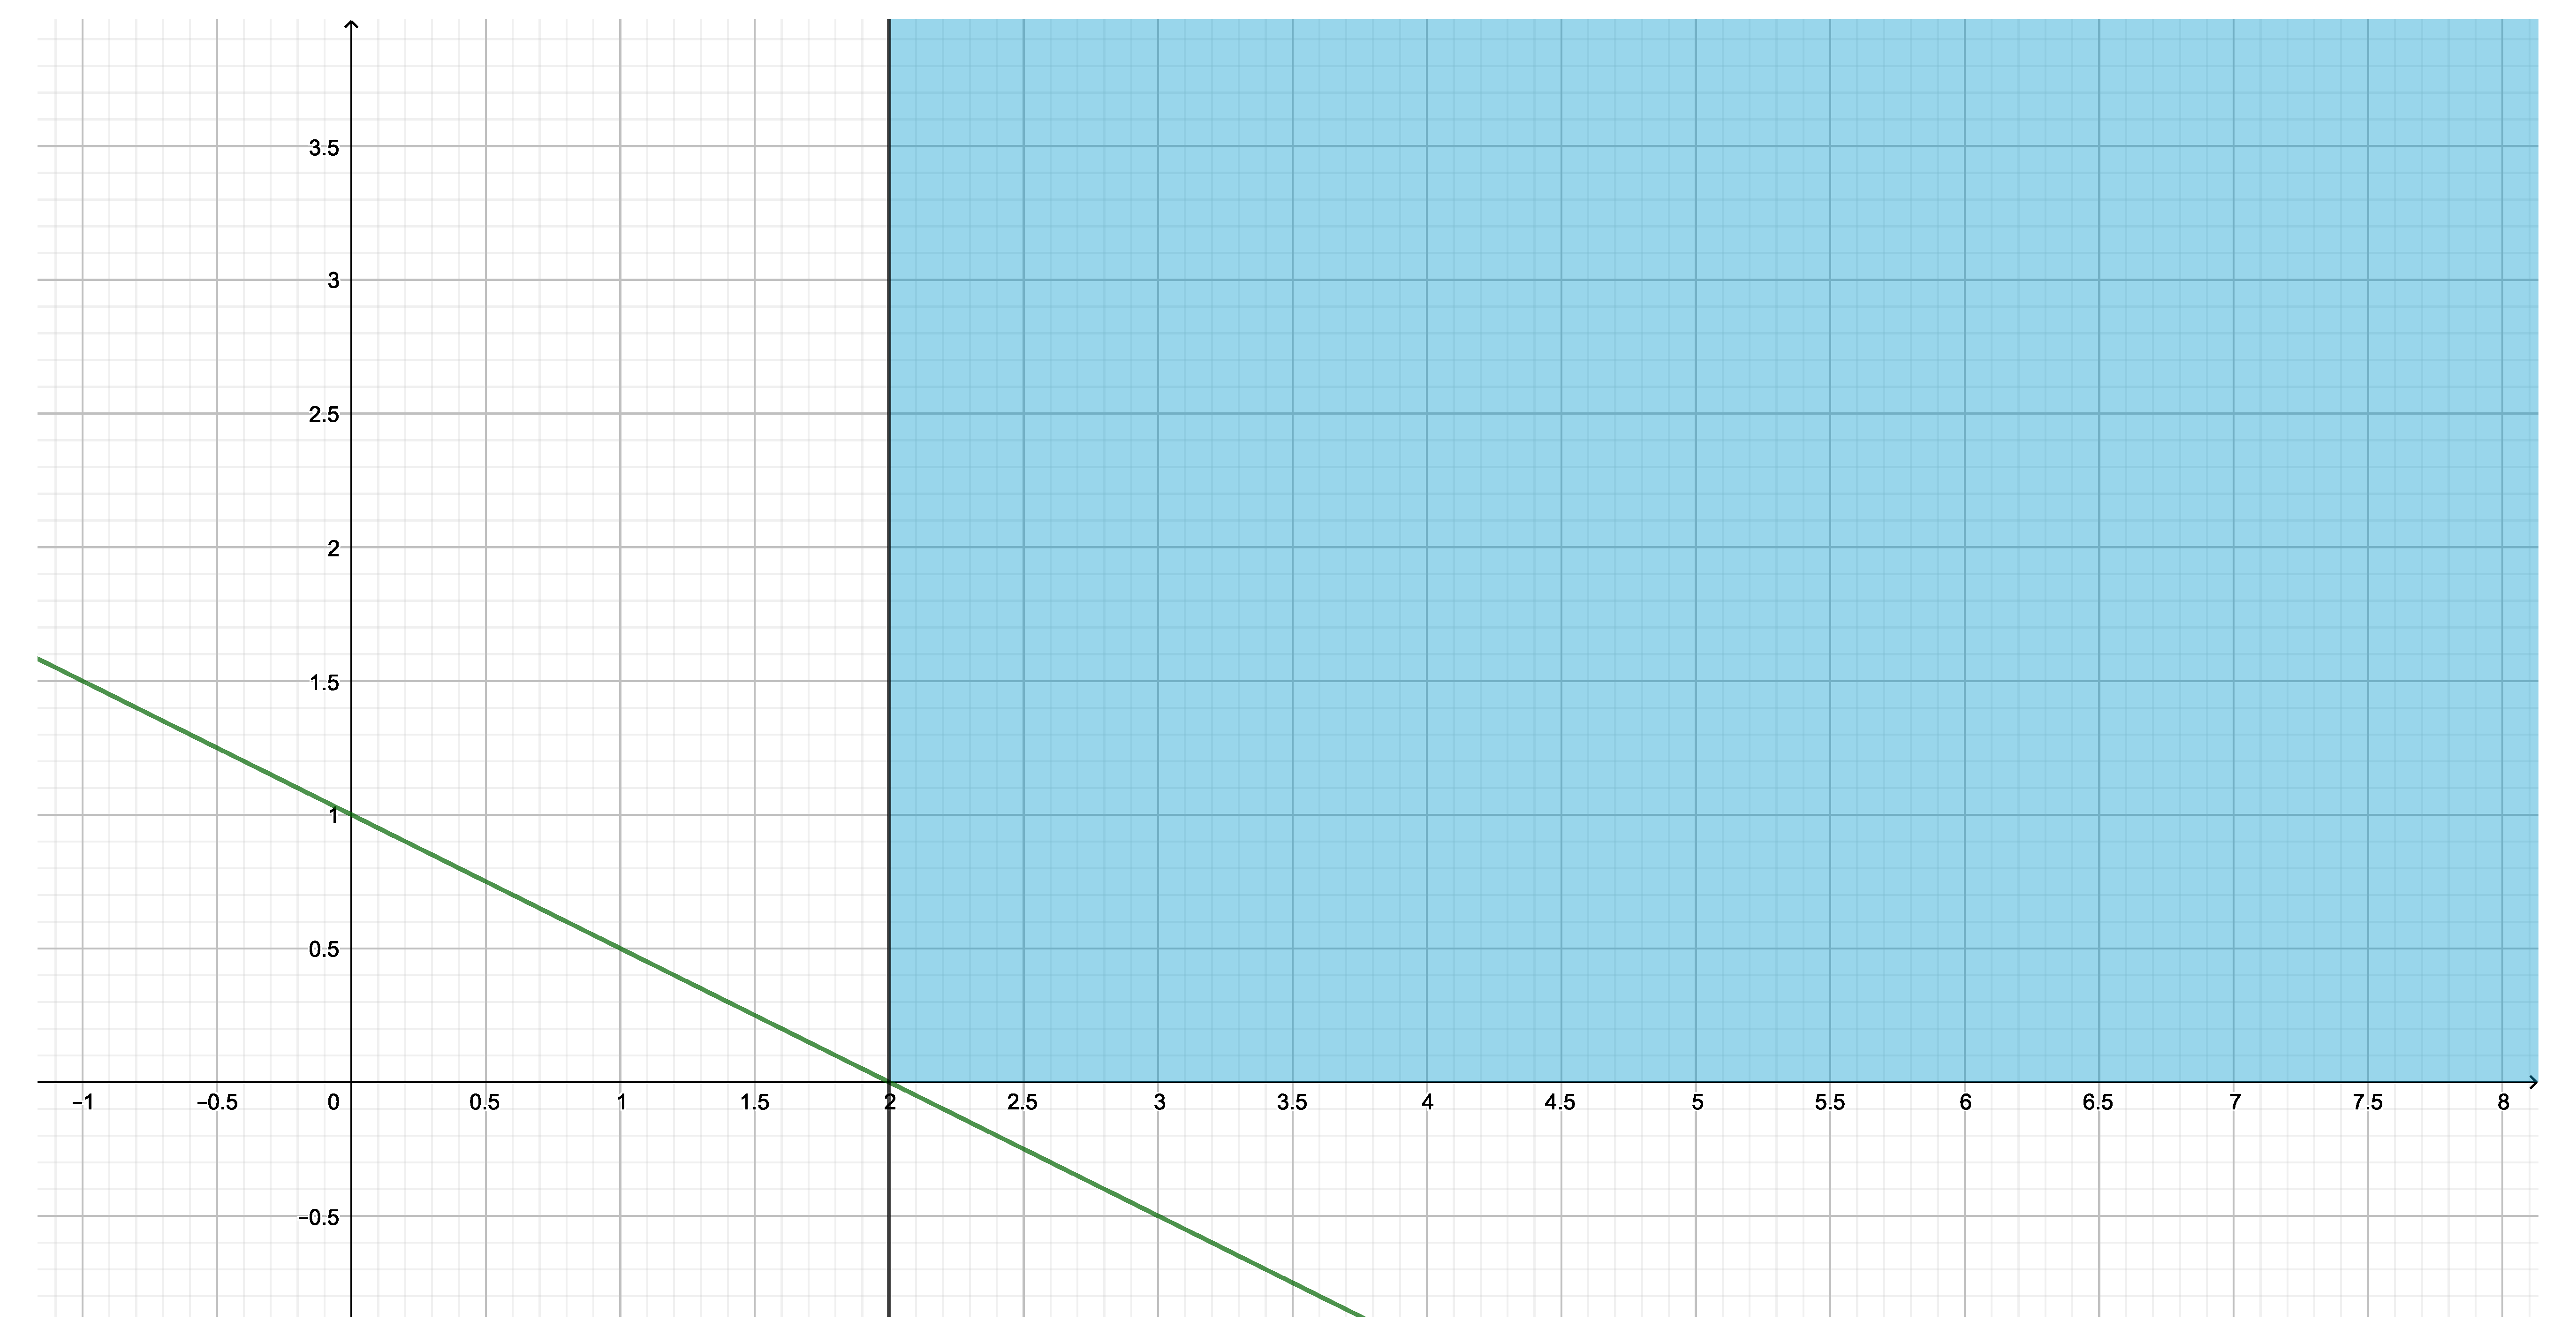
\includegraphics[width=0.5\textwidth]{fig2.pdf}
\end{figure}

\FloatBarrier


To solve the original problem, we can graph the feasible region in 3-D and use graph method to solve it. 


\end{enumerate}

\section*{Problem 1.4}
\begin{enumerate}
\item[a)]

No. Because it has absolute-value functions in the objective function.

\item[b)]
Let $x_i = x_i^+ - x_i^-$, $i = 1, 2, 3$, where $x_i^+, x_i^- \geqslant 0$. Then $|x_i| = x_i^+ + x_i^-$. Add one slack variable $\xi_1$ on the first constraint and the problem is reformed as

\begin{equation*}
\begin{aligned}
\text{Minimize} \quad & x_1^+ + x_1^- + 2x_2^+ + 2x_2^- - x_3^+ - x_3^- \\
\text{subject\  to} \quad & x_1^+ - x_1^- + x_2^+ - x_2^- - x_3^+ + x_3^- + \xi_1 = 10 \\
& x_1^+ - x_1^- - 3x_2^+ + 3x_2^- + 2x_3^+ - 2x_3^- = 12 \\
& x_i^+, x_i^- \geqslant 0, i = 1, 2, 3. \\
& \xi_1 \geqslant 0
\end{aligned}
\end{equation*}

\item[c)]

Use the similar technique as in (b), let $a_1 = x_1 - 5$ and $a_2 = x_2 + 4$. Then, $|x_1 - 5| = a_1^+ + a_1^-$ and $ |x_2 + 4| = a_2^+ + a_2^-$. 

Also, it is clear to see that

$$
x_1 = a_1 + 5 = a_1^+ - a_1^- + 5, \quad x_2 = a_2 - 4 = a_2^+ - a_2^- - 4.
$$

Plug above into the problem and get the following standard form.

\begin{equation*}
\begin{aligned}
\text{Minimize} \quad & a_1^+ + a_1^- + a_2^+ + a_2^- \\
\text{subject\  to} \quad & a_1^+ - a_1^- + a_2^+ - a_2^- + \xi_1 = 9 \\
& a_1^+ - a_1^- - 3a_2^+ + 3a_2^- - \xi_2 = -15 \\
& a_i^+, a_i^-, \xi_i \geqslant 0, i = 1, 2. 
\end{aligned}
\end{equation*}
\end{enumerate}


\section*{Problem 1.5}

Usually, the goal for this type of problems is either to minimize the total cost or to maximize the total profit. For this problem, we will consider maximize the price. Let the objective function be $f(x) = 15x_1 + 25 x_2$. Here $x_1$ and $x_2$ are the amount of Chip-1 and Chip-2 produced.

Consider the skilled and unskilled labor hours, and the available raw materials, the constraints are 
$$
3x_1 + 4x_2 \leqslant 100, \quad 2x_1 + 3x_2 \leqslant 70, \quad x_1 + 2x_2 \leqslant 30.
$$

Also, the amount of product should be non-negative. With the demand on the sales contract, we have
$$
x_1 \geqslant 0, \quad x_2 \geqslant 3.
$$

In conclusion, we can form the problem as a LP problem,

\begin{equation*}
\begin{aligned}
\text{Maximize} \quad & 15x_1 + 25 x_2\\
\text{subject\  to} \quad & 3x_1 + 4x_2 \leqslant 100 \\
&  2x_1 + 3x_2 \leqslant 70 \\
& x_1 + 2x_2 \leqslant 30 \\
& x_1 \geqslant 0, x_2 \geqslant 3.
\end{aligned}
\end{equation*}



\section*{Problem 1.6}

For this problem, our goal is to minimize the time(days) used for completing these 5 projects. 

Use matrix $T$ to express the given table. i.e., 

$$
T = 
\begin{pmatrix}
5 & 5 & 7 & 4 & 8 \\
6 & 5 & 8 & 3 & 7 \\
6 & 8 & 9 & 5 & 10 \\
7 & 6 & 6 & 3 & 6 \\
6 & 7 & 10 & 6 & 11
\end{pmatrix}
 = 
\begin{pmatrix}
t_A \\
t_B \\
t_C \\
t_D \\
t_E
\end{pmatrix}
$$

where $t_A, \dots, t_E$ are rows of $T$. Let $a, b, c, d, e \in \mathbb{R}^5$ (i.e. $a = (a_1, \dots, a_5)^T$) be variables and each of them shows the index of the project assigned to that person. For example, if $d = (0, 1, 0, 0, 0)^T$, it means person $D$ will work on project $\# 2$. 

Then our goal is to minimize the time spent on these projects.

$$
\text{Minimize} \quad t_Aa + t_Bb + t_Cc + t_Dd + t_Ee.
$$

Consider that one person is assigned to do one project, we have 

$$
\sum_{i = 1}^5 x_i = 1, \quad x \in \{a, b, c, d, e\}.
$$

What's more, every project has to be covered by one person and it leads to the following constraint,

$$
a_i + b_i + c_i + d_i + e_i = 1, \quad i = 1, \dots, 5.
$$

In conclusion, the integer linear programming problem is,

\begin{equation*}
\begin{aligned}
\text{Minimize} \quad & t_Aa + t_Bb + t_Cc + t_Dd + t_Ee \\
\text{subject\  to} \quad & \sum_{i = 1}^5 a_i = 1, \quad \sum_{i = 1}^5 b_i = 1, \quad \sum_{i = 1}^5 c_i = 1 \\
& \sum_{i = 1}^5 d_i = 1, \quad \sum_{i = 1}^5 e_i = 1 \\
& a_i + b_i + c_i + d_i + e_i = 1, \quad i = 1, \dots, 5 \\
& a_i, b_i, c_i, d_i, e_i \in \{0, 1\} , i = 1, \dots, 5.
\end{aligned}
\end{equation*}



\section*{Problem 1.7}

\begin{enumerate}
\item[a)]

Let $H_1, H_2$ and $H_3$ be the amount ship to HK from those three sources respectively. And let $h_1, h_2$ be output from HK to destinations respectively. Similar setting up for Taiwan.

\FloatBarrier

\begin{figure}[htpb]
  \caption{Problem 1.7}
  \centering
    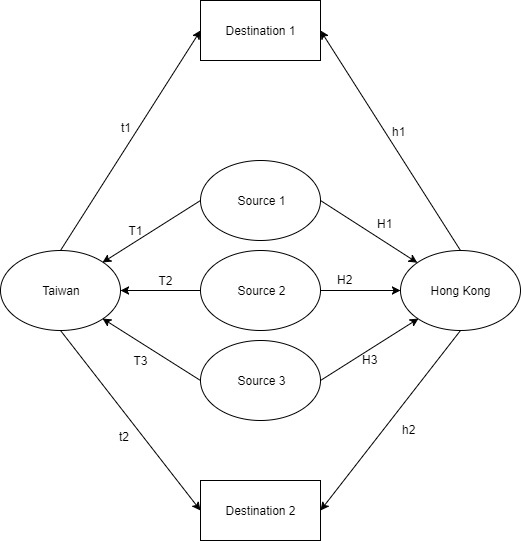
\includegraphics[width=0.5\textwidth]{fig3.jpg}
\end{figure}

\FloatBarrier

Consider the no-blands from each sources, and demands from destinations, the LP problem is,

\begin{equation*}
\begin{aligned}
\text{Minimize} \quad & 50H_1 + 90 H_2 + 70H_3 + 150h_1 + 180h_2 + 60T_1 + 95T_2 + 50 T_3 + 130t_1 + 200 t_2 \\
\text{subject\  to} \quad & T_1 + H_1 = 60 \\
& T_2 + H_2 = 45 \\
& T_3 + H_3 = 30 \\
& h_1 + t_1 = 80 \\
& h_2 + t_2 = 55 \\
& T_i, H_i \geqslant 0, i = 1, 2, 3 \\
& t_j, h_j \geqslant 0, j = 1, 2.
\end{aligned}
\end{equation*}

\item[b)]

Add a constraint in the LP problem of a).
$$
\sum_{i = 1}^3 H_i \leqslant 60.
$$


\item[c)]

We may want to try to add one more constraint based on b).
$$
\sum_{i = 1}^3 T_i \leqslant 50.
$$

This is fine. But after this we will see that there is no feasible solutions to the problem. The reason is that the output from HK and Taiwan will not meet the demands from destinations.



\item[d)]

(There might be different answers for this part.)

Part 1, we minimize the shipping cost from sources to HK and Taiwan. The amount of goods that the HK and Taiwan can deal with is less than the amount ordered from sources.

\begin{equation*}
\begin{aligned}
\text{Minimize} \quad & 50H_1 + 90 H_2 + 70H_3 + 60T_1 + 95T_2 + 50 T_3  \\
\text{subject\  to} \quad & T_1 + H_1 \leqslant 60 \\
& T_2 + H_2 \leqslant 45 \\
& T_3 + H_3 \leqslant 30 \\
& \sum_{i = 1}^3 H_i = 60 \\
& \sum_{i = 1}^3 T_i = 50 \\
& T_i, H_i \geqslant 0, i = 1, 2, 3 \\
\end{aligned}
\end{equation*}

Part 2, we minimize the shipping cost from HK and Taiwan to destinations. The amount of goods that the HK and Taiwan can deal with is less than the amount demanded.

\begin{equation*}
\begin{aligned}
\text{Minimize} \quad & 150h_1 + 180h_2 + 130t_1 + 200 t_2 \\
\text{subject\  to} \quad & h_1 + t_1 \leqslant 80 \\
& h_2 + t_2 \leqslant 55 \\
& h_1 + h_2 = 60 \\
& t_1 + t_2 = 50 \\
& t_j, h_j \geqslant 0, j = 1, 2.
\end{aligned}
\end{equation*}






\end{enumerate}

\end{document}